\chapter{Fault Tolerant Compressed Decoder}{
	% INTRO
	We decide to begin the creation of the FT IF stage from the Compressed Decoder (CD).
	The idea is to create a FT Compressed Decoder  manually, test it and then convert this architecture in a template.   
	This generic template will be written in Travulog and used to automatically convert IF stage sub-blocks in fault tolerant architecture.
	The conversion is described in the next chapter \ref{TravulogAndHtravulog}, here we focus on the design of the FT Compressed Decoder. \\
	
	
		The Compressed Decoder is a small, one input - three output, combinatorial sub-block of the if stage. 
		It is suitable to FT experimentation due to low input and output number, indeed  for TMR technique we need to add a voter for each output, so lower output means faster design time.\\
		
		The decision of the FT technique to use is linked to the final objective of the thesis, create a POW (Proof Of Work) of the Travulog/Htravulog Toolchain and create an FT IF stage at the same time.
		Therefore we decide to use the basic TMR technique plus a permanent error detector with alpha-counters.
		In this way we implement a FT if stage with the most used FT technique, this can be a good reference in the creation of Travulog template and speed up the understanding of the architecture, simplifying external approaches to the Travulog/Htravulog Toolchain.\\
		
		The first block we create is the \textbf{cv32e40p\_3voter}. 
		As you can see in \figref{fig:cv32e40p_voter}, the voter compare three inputs data in\_1\_i, in\_2\_i and in\_3\_i each other, the output \textit{voted\_o} is the result of the majority vote. 
		If all three inputs are different or in\_2\_i != in\_3\_i the output is equal to in\_1\_i, otherwise the output is in\_2\_i. 
		This type of voting give priority to in\_1\_i when all inputs are different, this is a non-significant choice for the final fault tolerance, indeed we can't know what input is correct if they are all different.\\
		
        We apply OR operation to each first, second and third element of block\_err\_o in order to find error in the corresponding replica, e.g., if the first replica have an error on is\_compressed\_o the second conf\_voter will have block\_err\_o=[1,0,0], while the other two conf\_voter will have block\_err\_o=[0,0,0], so we execute the OR between all block\_err\_o[0] and we find that occur an error in the first replica.\\
        
        The outputs of the OR are connected to the inputs of the Breakage Monitor, in this way each Breakage Monitor controls the corresponding replica. 
        When a replica is considered broken by the Breakage Monitor the corresponding bit of the is\_broken\_o vector is set to 1 and all conf\_voter will no longer consider the corresponding block. 
        In this case the compressed\_decoder\_ft became a duplex system and if one of the two replica failed the operation should be redone.\\
        
        
	    
	    \begin{figure}[H]
    		\centering
    		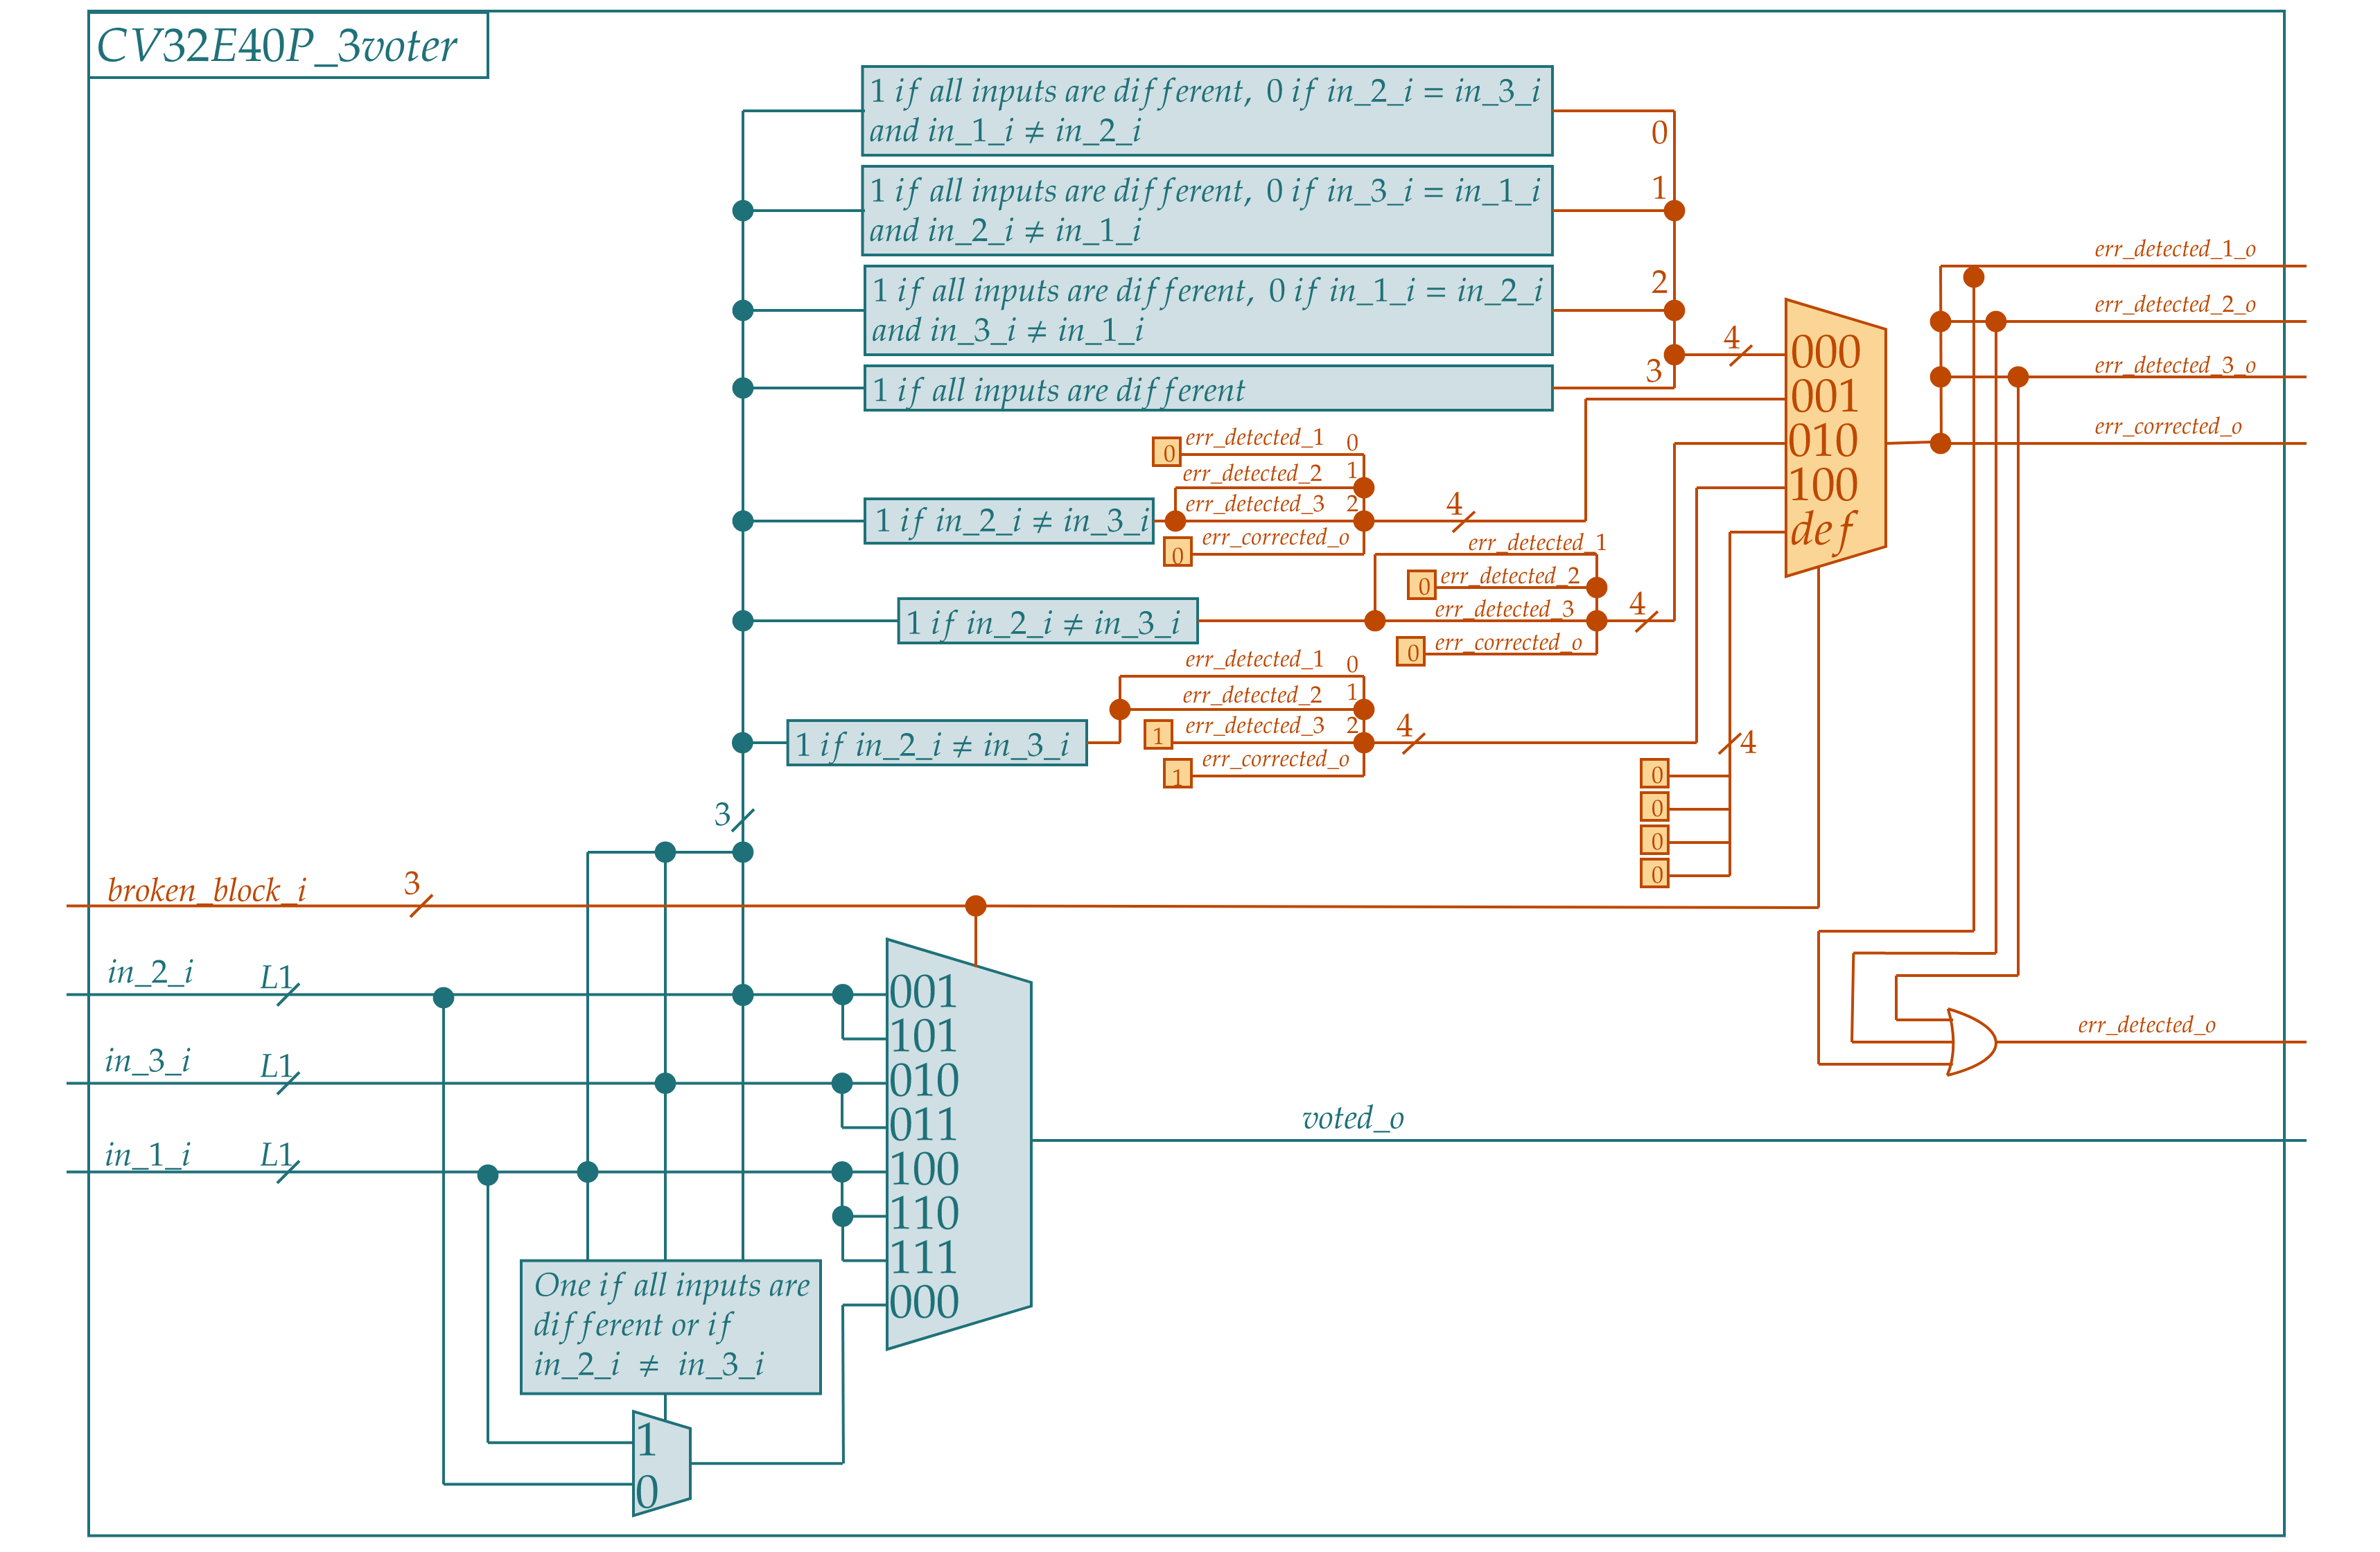
\includegraphics[width=1.1\textwidth,center]{./images/cv32e40p_3voter.png}
    		\caption{This is the voter used in the fault tolerant architecture.}
    		\label{fig:cv32e40p_voter}
    	\end{figure} 	
    	
    	The designed voter have also a three bit input called \textit{broken\_block\_i}, each bit refers to a block, 0 means that the block work properly while 1 means that it has permanent error.
        For example [0,0,0] means that all input signals came from block without permanent error, instead [0,1,0] means that the second block have a permanent error.
        
        \textit{broken\_block\_i} allows the discarding of input signals from permanent faulty blocks.
        Indeed the multiplexer that decide voted\_o is controlled by the broken\_block\_i, e.g., when in\_1\_i came from a permanent faulty block is automatically selected in\_2\_i as output, so the system became a duplexer.\\
        
        In addition to the voting part there is some logic that indicate when there is a faulty input and when it is corrected.
        \textit{err\_detected\_1\_o}, \textit{err\_detected\_2\_o} and \textit{err\_detected\_3\_o} are one if the corresponding input signals in\_1\_i, in\_2\_i and in\_3\_i have a transient fault. When the input signal in\_x\_i is permanent faulty the corresponding output  err\_detected\_x\_o is 0, the remaining two output err\_detected\_y\_o and err\_detected\_z\_o will be both 1 if the corresponding inputs are different because we can't know which is the correct input.
        
        The err\_corrected\_o signal is one if the detected error has been corrected and it is 0 if all input are different.\\
        
        The cv32e40p\_3voter block can be use for single dimension array changing the L1 parameter, this parameter change the dimension of in\_x\_i and voted\_o signals, e.g., if you have three 32-bit signals to compare set L1 to 32 to use the voter.\\
        
        
        In order to enable triple voter configuration, we create the \textbf{cv32e40p\_conf\_voter}.
        This block can be used as a simple voter if TOUT is set to 0 \figref{fig:cv32e40p_conf_voter}  or as a triple voter if TOUT is set to 1 \figref{fig:cv32e40p_conf_voter_tout1} .
        The external interface of the conf\_voter is the same of the voter apart for triple input called to\_vote\_i and triple output. 
        If TOUT is 0 the  output of the voter is connected to the first element of voted\_o, the other two elements aren't connected and don't exist in the final layout. The three err\_detected signals of voter are grouped in block\_err\_o, so basically if TOUT is 0 the conf\_voter is about equal to the cv32e40p\_3voter.
        
        Instead if TOUT is 1, the conf\_voter creates three instances of the voter, each voter votes independently the three inputs. The three outputs are connected to voted\_o signal. 
        Finally the status signals are voted and sent to output.
        
        As you can see the external interface of the conf\_voter remain the same if you change TOUT, this allow a wide use of the block.\\
        
	    \begin{figure}[H]
    		\centering
    		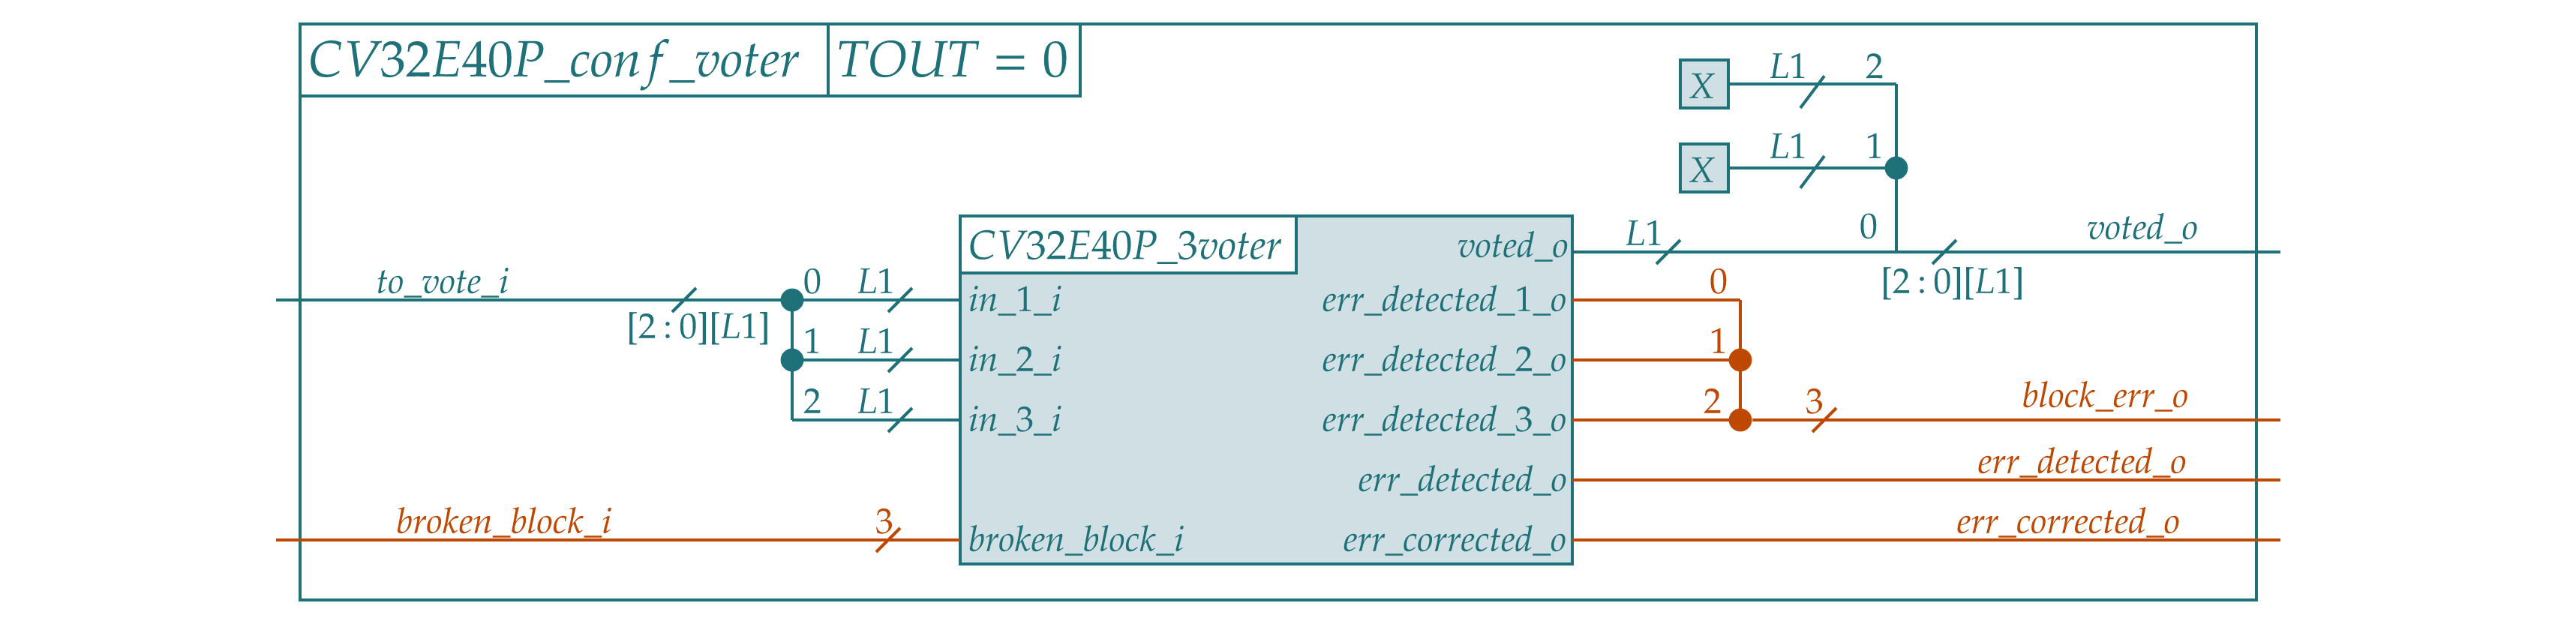
\includegraphics[width=1.3\textwidth,center]{./images/cv32e40p_conf_voter.png}
    		\caption{Configurable voter, with TOUT=0, a single voter.}
    		\label{fig:cv32e40p_conf_voter}
    	\end{figure} 	
    	
	    \begin{figure}[H]
    		\centering
    		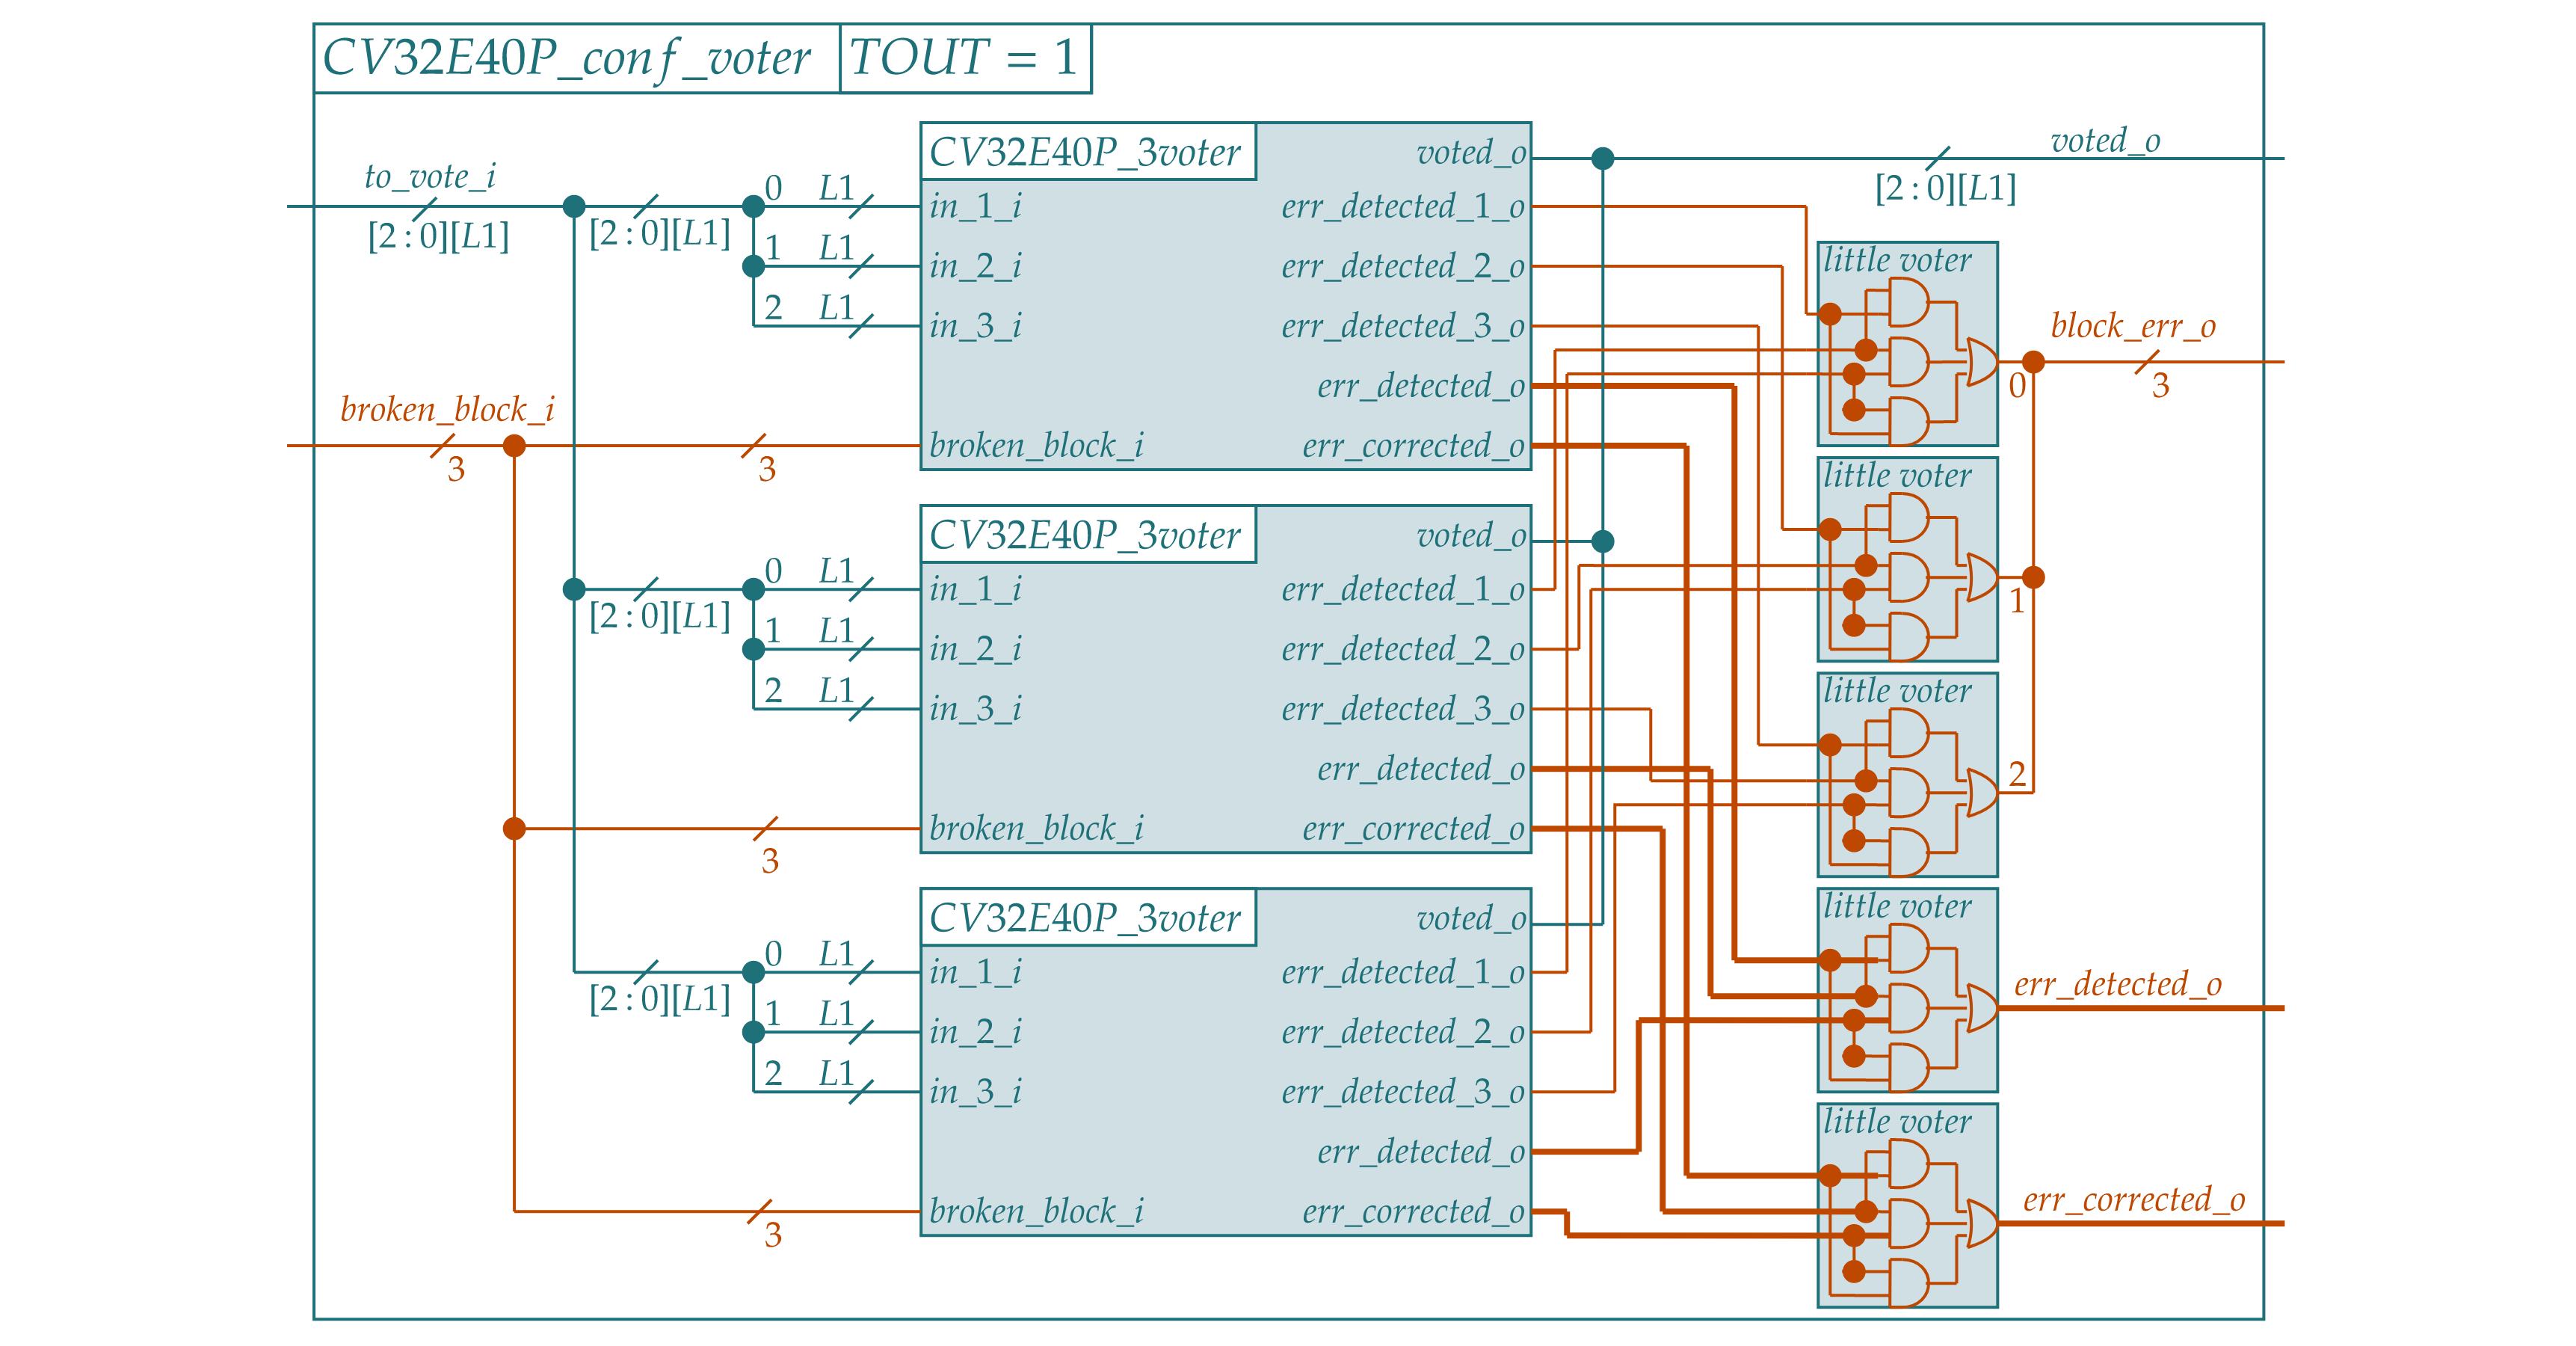
\includegraphics[width=1.3\textwidth,center]{./images/cv32e40p_conf_voter_tout1.png}
    		\caption{Configurable voter, with TOUT=1, a triple voter.}
    		\label{fig:cv32e40p_conf_voter_tout1}
    	\end{figure} 	
	
	
	    The third block is the \textbf{cv32e40p\_breakage\_monitor} in \figref{fig:cv32e40p_breakage_monitor}. 
	    Each time the  Breakage Monitor is instanced we should associate it to one replica inside a NMR structure, in our case we have a TMR and so we will use three Breakage Monitor, one for each replica of the Compressed Decoder.
	    Each time that the associate block have an error err\_detected\_i should be asserted, this increase reg\_count\_q by INCREMENT value.
	    Instead if err\_detected\_i is 0 reg\_count\_q is decreased by DECREASE value, both INCREMENT and DECREASE are SV parameters that can be changed.
	    When reg\_count\_q is higher than the  BREAKING\_THRESHOLD is\_broken\_o is asserted, this activate the clock gating which freeze the block maintaining is\_broken\_o to 1. The block can also be set broken using the set\_broken\_i input signal.\\
	    
	    This mechanism of increment and decrease allow to discard transient error because their frequency is really low, so for one increment there are thousands of decrease. 
	    Instead when exist a permanent error typically it appears more frequently and so the increase rate is higher.
	    Anyway you can steer INCREMENT, DECREASE and BREAKING\_THRESHOLD parameters in order to fit the error rate of your application. 
	    The SV module allow also the change of the register size: INC\_DEC\_BIT is the number of bit for register that contain INCREMENT and DECREASE variable, instead COUNT\_BIT is the number of bit of reg\_count register.
	    Naturally we fit the number of bit with the parameters value.\\
	    
	    \begin{figure}[H]
    		\centering
    		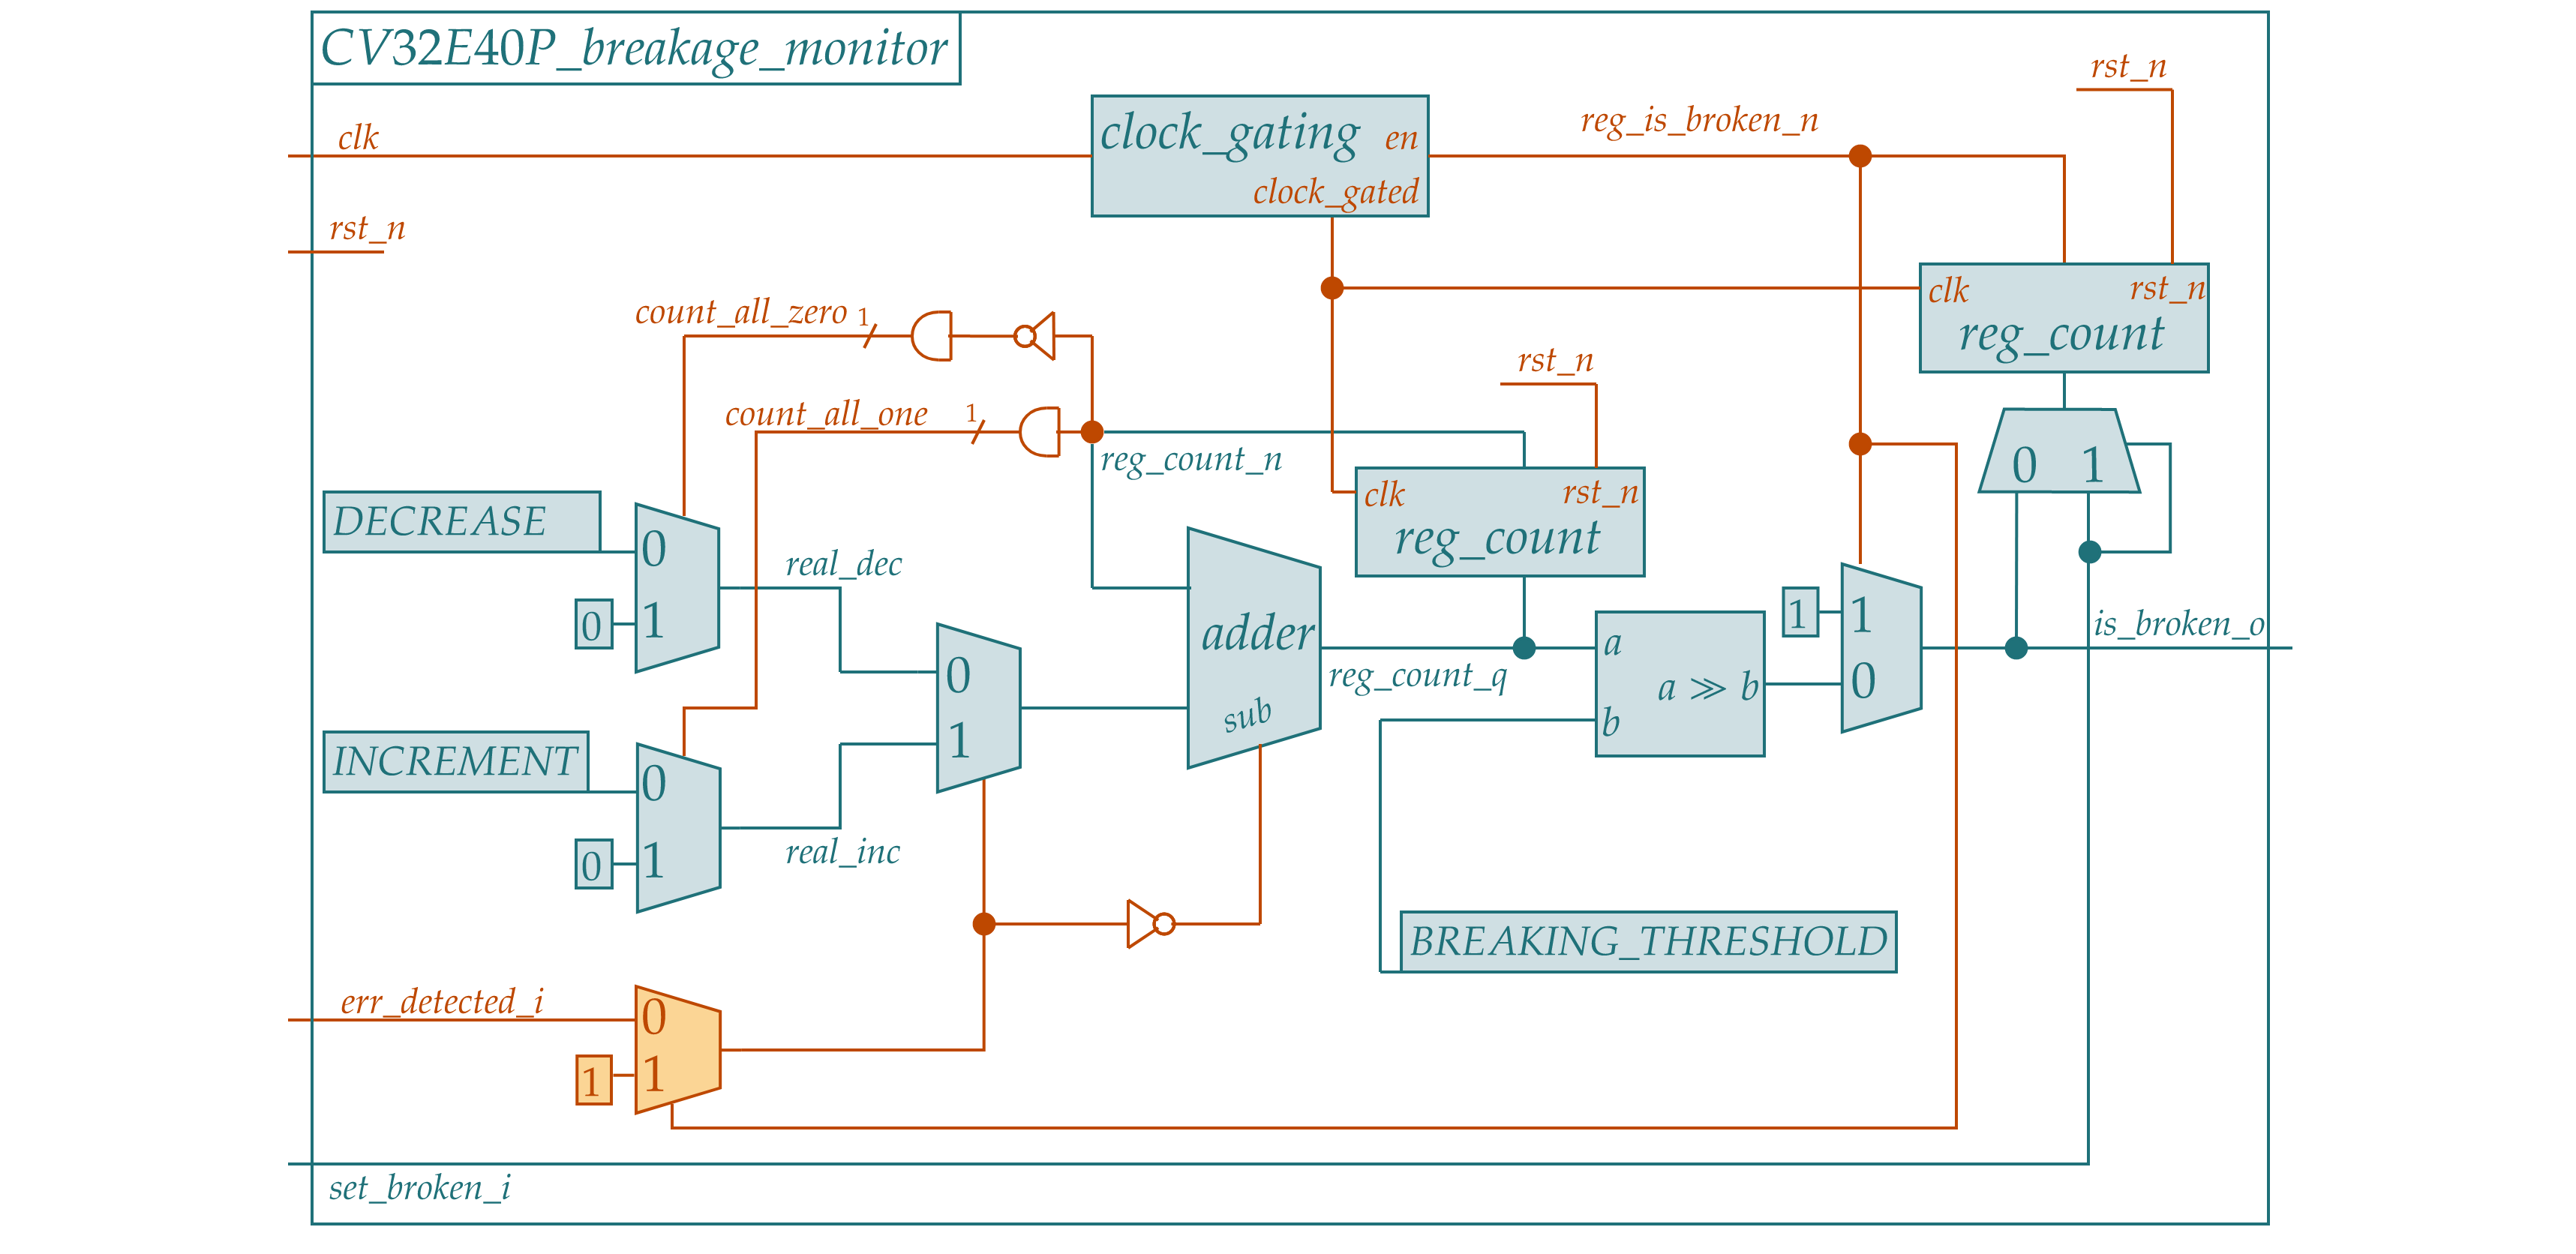
\includegraphics[width=1.3\textwidth,center]{./images/cv32e40p_breakage_monitor.png}
    		\caption{Breakage Monitor to detect permanent errors.}
    		\label{fig:cv32e40p_breakage_monitor}
    	\end{figure} 	
		
		The last block is the \textbf{cv32e40p\_compressed\_decoder\_ft} in \figref{fig:cv32e40_compressed_decoder_ft}, here we use all previous blocks to create a new FT configurable compressed decoder.
		On the right there are three replicas of the Compressed Decoder, the nine outputs are grouped by name so all instr\_o outputs are connected to instr\_o\_to\_vote, is\_compressed\_o outputs are connected to is\_compressed\_o\_to\_vote and finally illegal\_instr\_o outputs are connected to illegal\_instr\_o\_to\_vote.
		
		These *\_to\_vote signals are connected to the relative conf\_voter, as you can see in \figref{fig:cv32e40_compressed_decoder_ft} the first conf\_voter have three voter inside due to TOUT=1, this is an example of setting.
		Each conf\_voter have the block\_err\_o output, the first bit of these signals is referred to the first replica error, the second bit to the second replica and the third to the third replica. The first block\_err\_o signal is referred to errors on instr\_o, the second block\_err\_o to is\_compressed\_o and the third to illegal\_instr\_o.
		
	    We apply OR operation to block\_err\_o in order to find if there is at least an error in a each replica, we send this three signals to the Breakage Monitor to that check the presence of permanent errors.
	     
		
	    \begin{figure}[H]
    		\centering
    		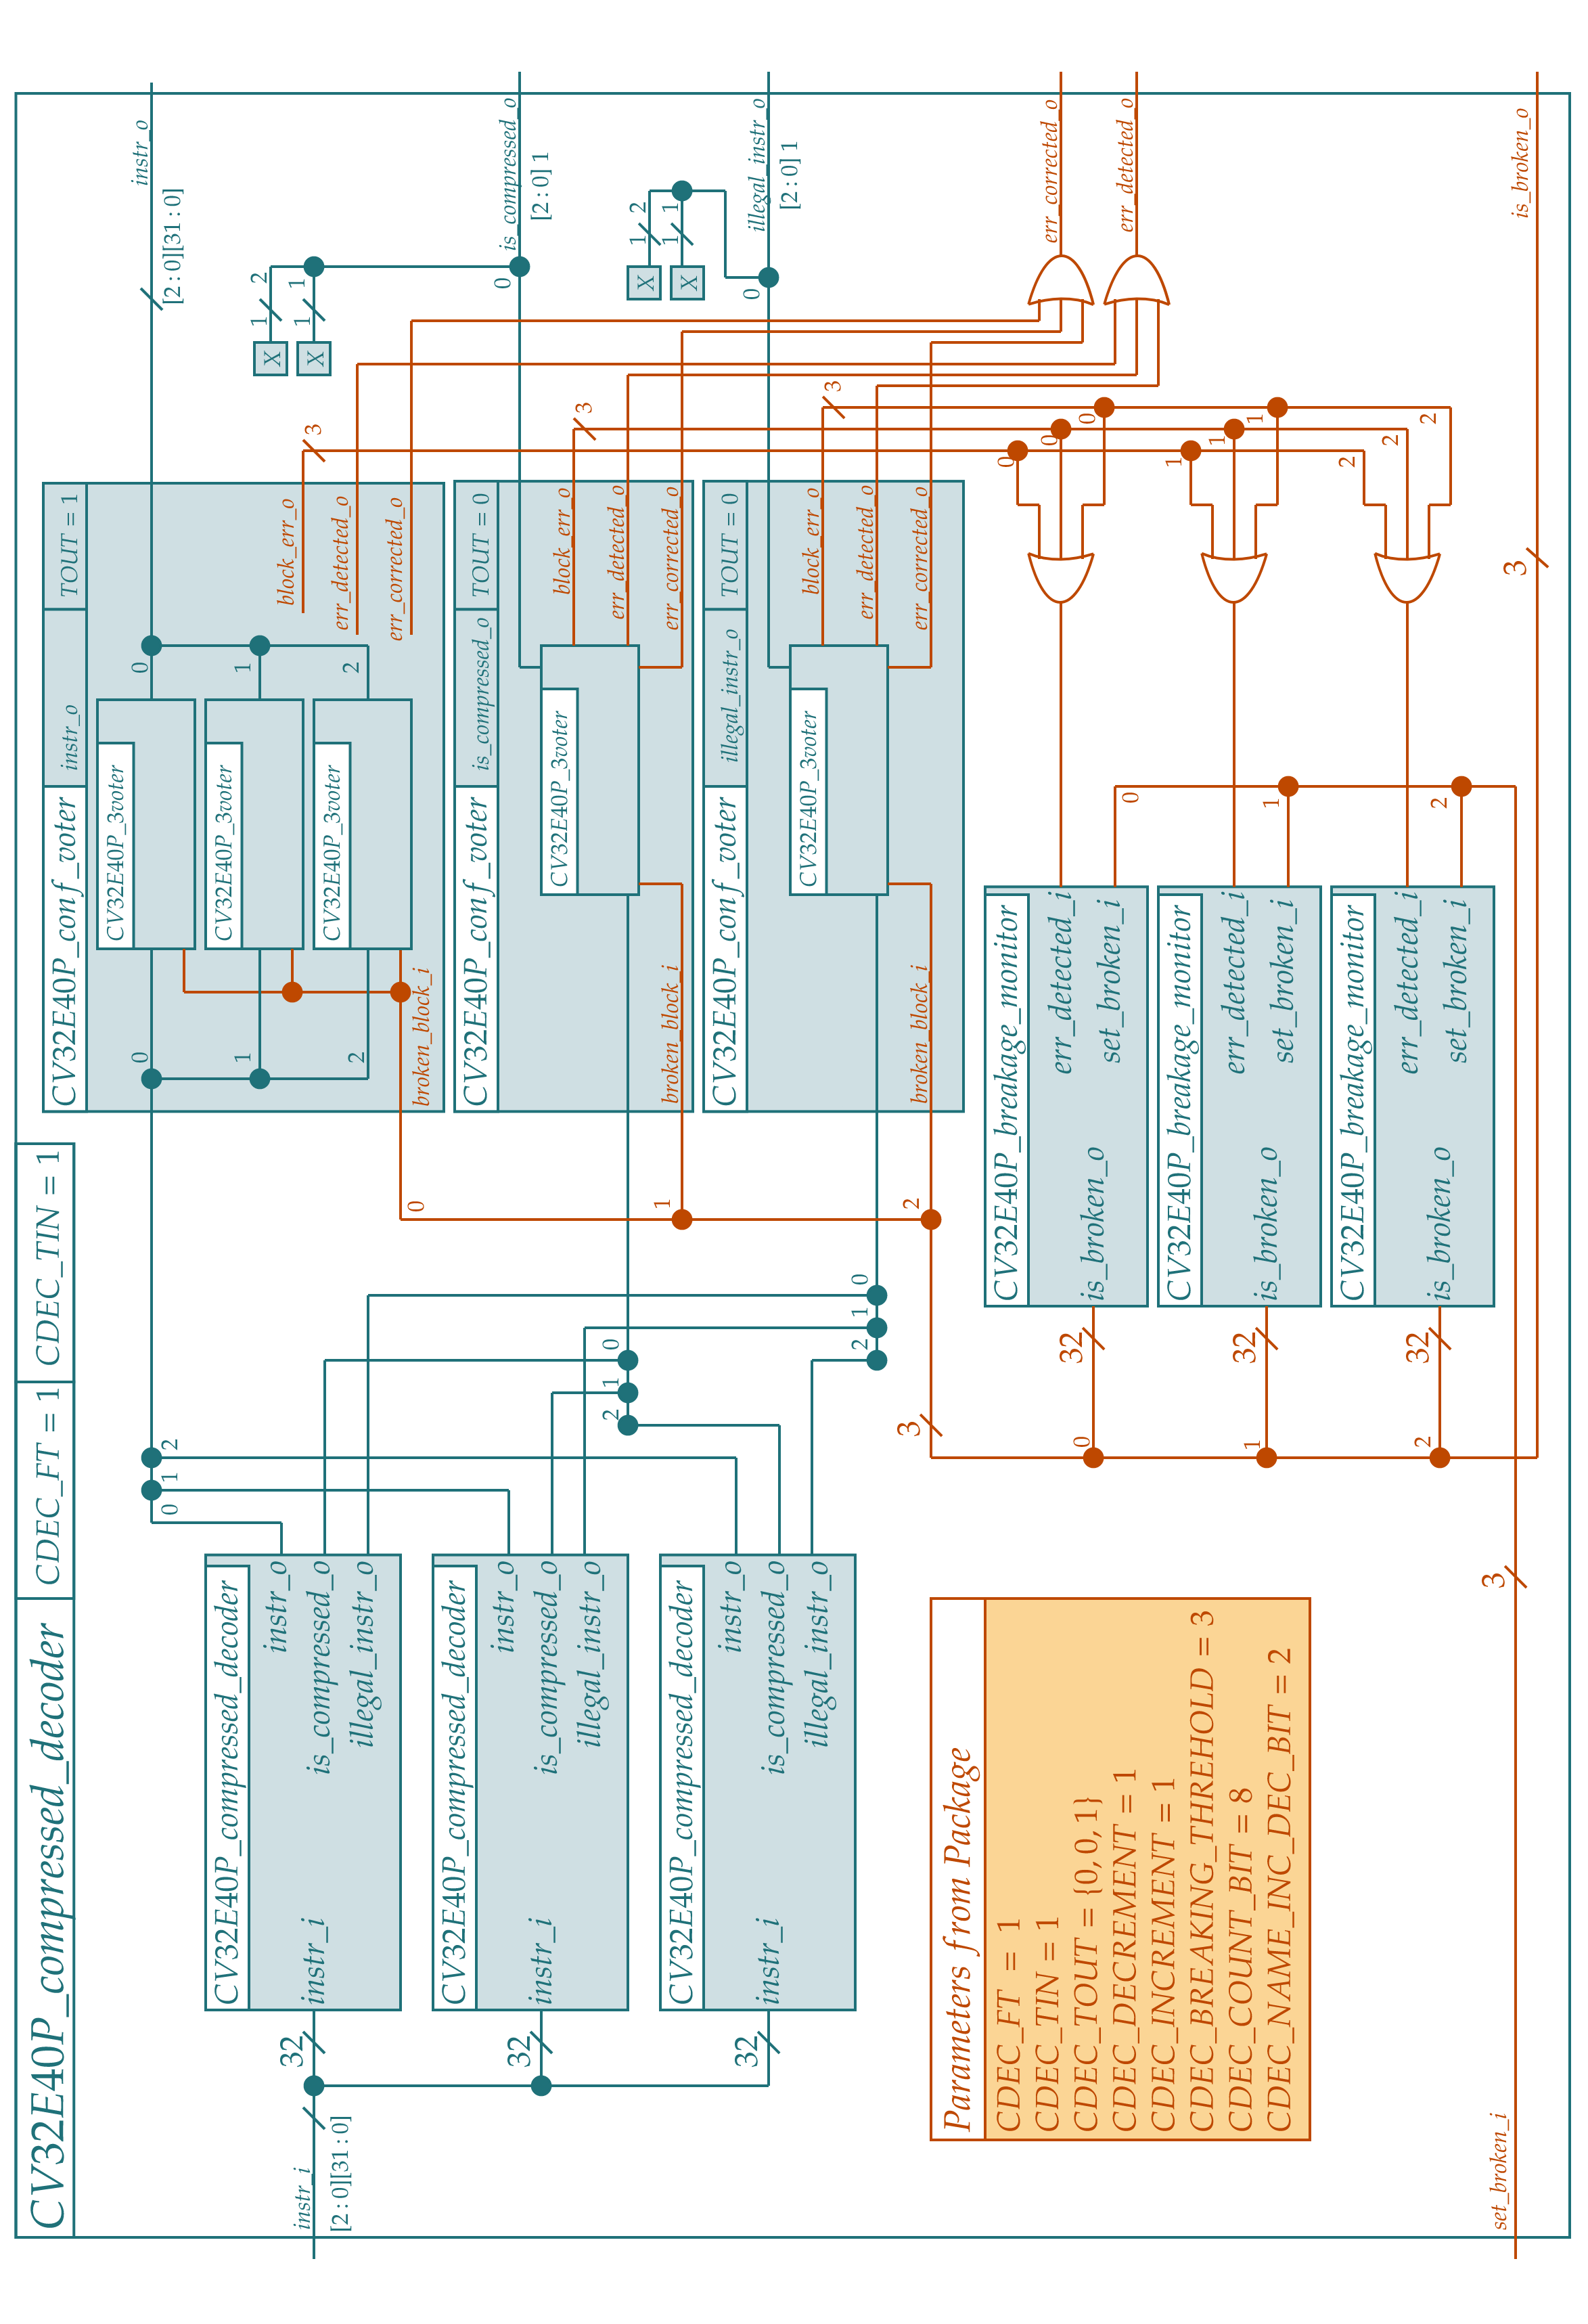
\includegraphics[width=0.95\textwidth,center]{./images/cv32e40p_compressed_decoder_ft.png}
    		\caption{A possible configuration of the Configurable Compressed Decoder.}
    		\label{fig:cv32e40p_compressed_decoder_ft}
    	\end{figure} 	
    	 Each Breakage Monitor is related to the corresponding replica and we send their output to conf\_voters, in this way when occur a permanent error in one replica their output are discarded, in this case the system became a duplexer. 
    	 
    	 set\_broken\_i is a three bit signal used to set broken a replica, at the same time exist the is\_broken\_o signal used to communicate if there are permanent broken block.
    	 
    	 These two signals can be used to save internal replicas status in some non-volatile memory ( e.g., CSR registers) and use these information to reload replicas status inside the FT compressed decoder if the system is rebooted.\\
    	 
    	 Finally we have err\_corrected\_o and err\_detected\_o that communicate when an error occurs and if it has been corrected.
    	 These two signals can be used at high level to check architecture integrity and eventually indicate if the system should be replaced due to high error rate.\\
    	 
    	 In the Parameters From Package table there are all SV parameters that can be changed to configure the block. So the feature of the block are:
    	 \begin{itemize}
    	     \item \textbf{Fault Tolerance:} If CDEC\_FT=1 is used TMR technique as you see in the picture, otherwise is used only one Compressed Decoder and the cv32e40p\_compressed\_decoder\_ft became the basic cv32e40p\_compressed\_decoder.
    	     \item \textbf{Triple Input:} When you set CDEC\_TIN=1 should be provided three instr\_i inputs, each input is connected to the corresponding compressed decoder, otherwise is used only one input equal for each replica. This feature is useful if the previous block implement triple voter configuration. 
    	     \item \textbf{Triple Output:} Each bit of CDEC\_TOUT corresponds to a conf\_voter and so to an output, the MSB is the last bit and it corresponds to the first output. The order of the output corresponds to the appearance order in the port declaration od the cv32e40p\_compressed\_decoder. When a bit of the CDEC\_TOUT is 1 the corresponding conf\_voter implement a triple voter, this means that the corresponding output will have three valid signals from triple voter.
    	     \item \textbf{Permanent Error Settings:} The remaining parameters are used to set the Breakage Monitor parameters, all Breakage monitor will have the same configuration.
    	 \end{itemize}
    	 
    	 As we have seen this block is highly configurable, due to triple input - output option both input and output signals are triplicated in the port declaration. 
    	 
    	 Anyway in some configuration not all input and output signals are connected, this means that care must be taken in the block connection and parameters configuration.
	    
	%section{Verification}{
	
	%}% end of
}